% ----------------------------------------------------------
% Projeto
% ----------------------------------------------------------
\chapter[Projeto de implementação]{Projeto de implementação}\label{chap:projeto}

Nesse capítulo apresentamos a estrutura, arquitetura e funcionalidades do projeto abordado realizado no trabalho. 
Em primeiro momento foi feita uma análise dos requisitos necessários, para que então pudéssemos organizar todas as funcionalidades dentro do protótipo da aplicação e por fim projetar a arquitetura do \textit{software} e a modelagem do banco de dados.

\section{Análise de Requisitos}

Dois tipos de requisitos foram levantados para a implementação do projeto: Requisitos Funcionais (RF), que são aqueles que definem as funcionalidades e como o \textit{software} se comporta; e os Requisitos Não-Funcionais (RNF), que são responsáveis por especificar quesitos mais técnicos do \textit{software}, como tecnologias, segurança e desempenho. 

Para definição dos RF, foram analisados programas no estado da arte das duas categorias abordadas (videoconferência e atendimento ao consumidor) e coletadas funcionalidades consideradas importantes. Os RNF foram definidos a partir de estudos de aplicações Web modernas, com exceção do WebRTC que foi definido desde o principio. Requisitos funcionais serão apresentados com um diagrama de casos de uso, sendo cada caso um requisito. 

Os RNF levantados são os seguintes (os itens 11, 12 e 13 foram baseados no trabalho \cite[Sec.~4.3.1]{webrtcquality}):
\begin{itemize}
	\item RNF 01: Utilizar a linguagem JavaScript.
    \item RNF 02: Arquitetura REST para API.
    \item RNF 03: Arquitetura com WebSockets para estabelecer a conexão P2P.
    \item RNF 04: Utilizar plataforma NodeJS para o servidor.
    \item RNF 05: Utilizar \textit{framework} ExpressJS para API.
    \item RNF 06: Utilizar \textit{framework} SocketIO para suporte a WebSocket.
    \item RNF 07: Utilizar \textit{framework} ReactJS para renderizar interface no navegador.
    \item RNF 08: Utilizar PostgreSQL como gerenciador de banco de dados.
    \item RNF 09: Suporte a dispositivos móveis.
    \item RNF 10: Utilização de WebRTC para videoconferência.
    \item RNF 11: A taxa de transmissão deve estar acima de 1.0 Mbps.
    \item RNF 12: Porcentagem de perda de pacotes não deve ultrapassar o máximo de 10\%.
    \item RNF 13: Limite da latência da comunicação de 1000 milisegundos.
\end{itemize}

Os RF levantados são representados como casos de uso na \autoref{fig:usecases}.

\begin{figure}[ht!]
	\centering
    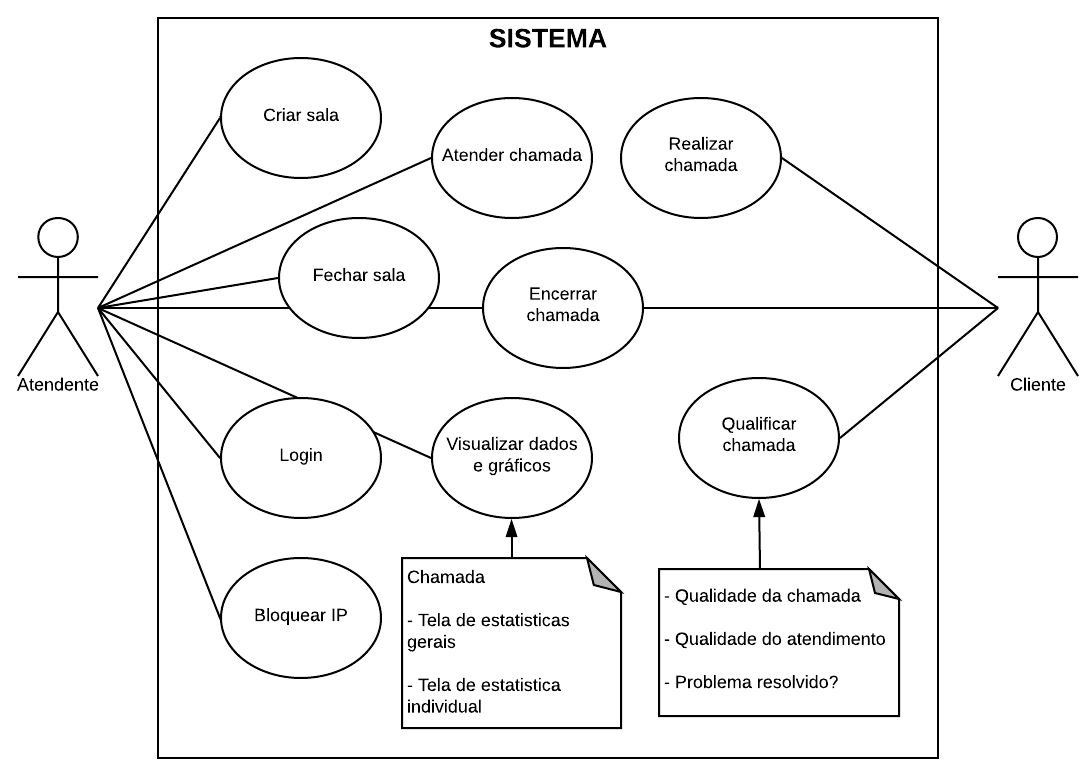
\includegraphics[scale=0.9]{figures/usecases.png} 
	\caption{Requisitos Funcionais do sistema representados por casos de uso}
	\label{fig:usecases}
\end{figure}

\newpage
\section{Protótipos de tela}

\subsection{Login}

A tela inicial da aplicação é a de login (ver \autoref{fig:login_prototype}), constituída de um pequeno formulário de autenticação e um logo no canto esquerdo. 

\begin{figure}[ht!]
	\centering
    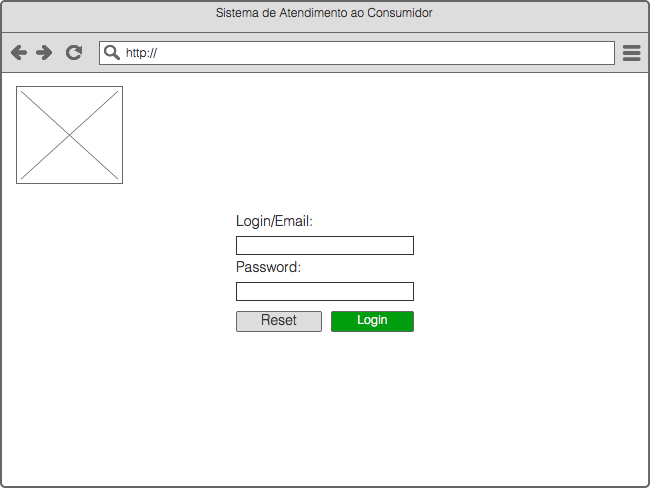
\includegraphics[scale=0.4]{figures/prototypes/login.png} 
	\caption{Tela de login}
	\label{fig:login_prototype}
\end{figure}

Como nenhum cliente necessita de cadastro para realizar chamadas, a tela está disponível somente para os atendentes entrarem no gerenciamento de tickets. 

 Ao inserir os dados corretamente o atendente é redirecionado para a lista de tickets (ver \ref{subsec:ticket_management}). Caso contrário, um erro é mostrado no formulário.

\subsection{Gerenciamento de tickets}\label{subsec:ticket_management}

A tela de Gerenciamento de Tickets é a primeira tela do sistema de atendimento. Podemos observar nas figuras \ref{fig:support_statistics}, \ref{fig:ticket_statistics} e \ref{fig:call_statistics} 
que a interface é constituída de uma barra lateral na esquerda e o conteúdo principal à direita. 

O conteúdo a ser mostrado na direita dependerá do contexto da aplicação e de onde o usuário está no momento. Temos três situações diferentes que podem acontecer.

De inicio, temos a tela de estatísticas de tickets relacionados ao atendente (\autoref{fig:support_statistics}). Essa tela aparece no conteúdo principal quando o usuário não tem nenhum ticket selecionado. Ela reúne informações de todos os atendimentos feitos pelo usuário autenticado, como:

\begin{itemize}
  \item Número total de chamadas;
  \item Tempo total de chamada;
  \item Média de qualidade de atendimento;
  \item Média de qualidade de ligação; e
  \item Porcentagem de problemas resolvidos.
\end{itemize}

\begin{figure}[ht!]
	\centering
    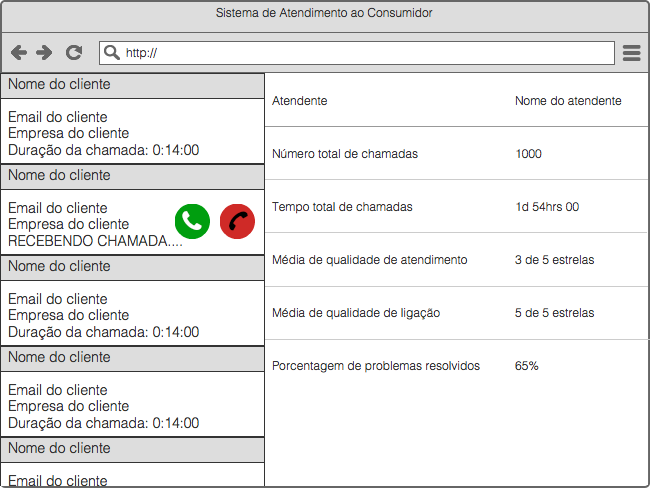
\includegraphics[scale=0.4]{figures/prototypes/support-statistics.png} 
	\caption{Tela de estatísticas do atendente}
	\label{fig:support_statistics}
\end{figure}

A segunda tela (\autoref{fig:ticket_statistics}) diz respeito a informações sobre um ticket específico que está selecionado.

É importante frisar que o item selecionado é de um atendimento já encerrado, pois o conteúdo é diferente e mostra informações adicionais sobre  a qualidade da chamada e algumas vezes até a opinião do cliente atendido, se fornecida pelo mesmo.

Os dados presentes são:

\begin{itemize}
  \item Nome do cliente e e-mail do cliente;
  \item Empresa, se existir;
  \item Descrição do problema;
  \item Duração do atendimento;
  \item Qualidade da ligação;
  \item Qualidade do atendimento; e se
  \item O problema foi resolvido.
\end{itemize}

\begin{figure}[!htb]
	\centering
    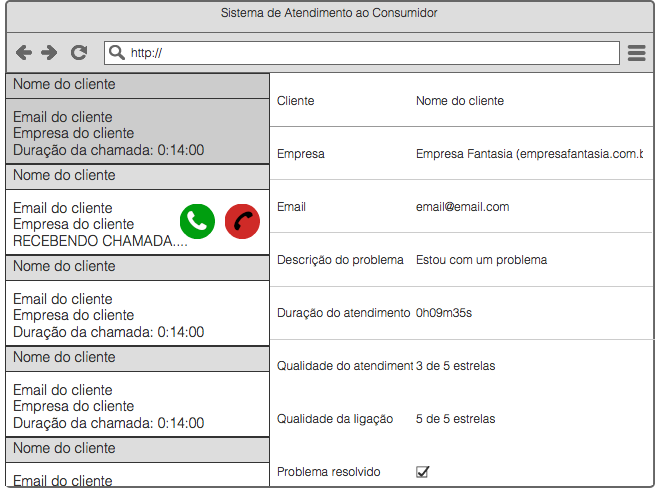
\includegraphics[scale=0.4]{figures/prototypes/ticket-statistics.png} 
	\caption{Tela de estatísticas de um ticket encerrado}
	\label{fig:ticket_statistics}
\end{figure}

Por último, temos na \autoref{fig:call_statistics} a tela que mostra o conteúdo de um ticket em aberto, ou seja, que o cliente está requisitando a chamada no momento. Nessa tela são exibidas as seguintes informações:

\begin{itemize}
	\item Nome e-mail do cliente;
    \item Empresa, se existir;
    \item Descrição do problema; e
    \item Botões de aceitar ou recusar chamada.
\end{itemize}

\begin{figure}[ht!]
	\centering
    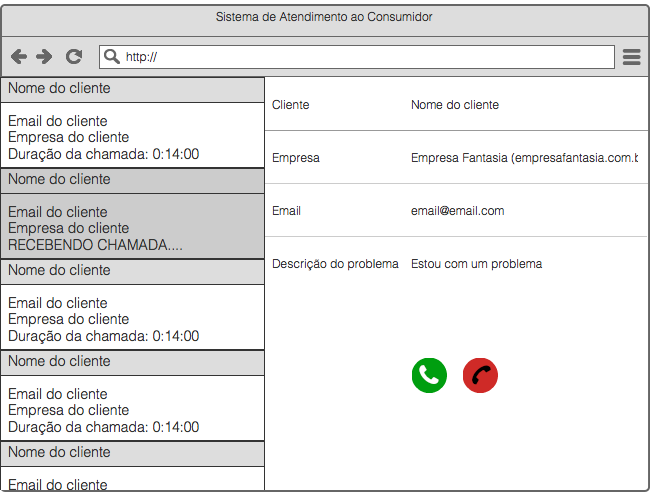
\includegraphics[scale=0.4]{figures/prototypes/call-statistics.png} 
	\caption{Tela de estatísticas de uma requisição de chamado}
	\label{fig:call_statistics}
\end{figure}

\subsection{Plugin para videoconferência}

O sistema de atendimento fornece aos seus usuários uma maneira de integrar um videochat no site da empresa através de um plugin. Esse plugin é feito a partir de tecnologias disponíveis no navegador (ou seja, não requer outros plugins, como Flash). O chat fornece três interfaces diferentes:

\begin{itemize}
  \item Plugin fechado e com um botão para abrir localizado no canto direito inferior;
  \item Plugin aberto com um formulário de requisição de atendimento; e
  \item Plugin aberto após encerramento de chamada com botões para qualificar atendimento.
\end{itemize}

\subsection{Tela de videoconferência}

Consiste na interface que compreende a funcionalidade principal do sistema de atendimento. Foi separada em um módulo e está presente tanto na aplicação voltada para atendentes quando no videochat integrado no site do cliente. A tela contém os seguintes itens:

\begin{itemize}
 \item Imagem da câmera do cliente sendo atendido;
 \item Imagem da câmera do atendente prestando atendimento;
 \item Botões para encerrar chamada e silenciar microfone;
 \item Dados sobre o presente atendimento.
\end{itemize}

\begin{figure}[ht!]
	\centering
    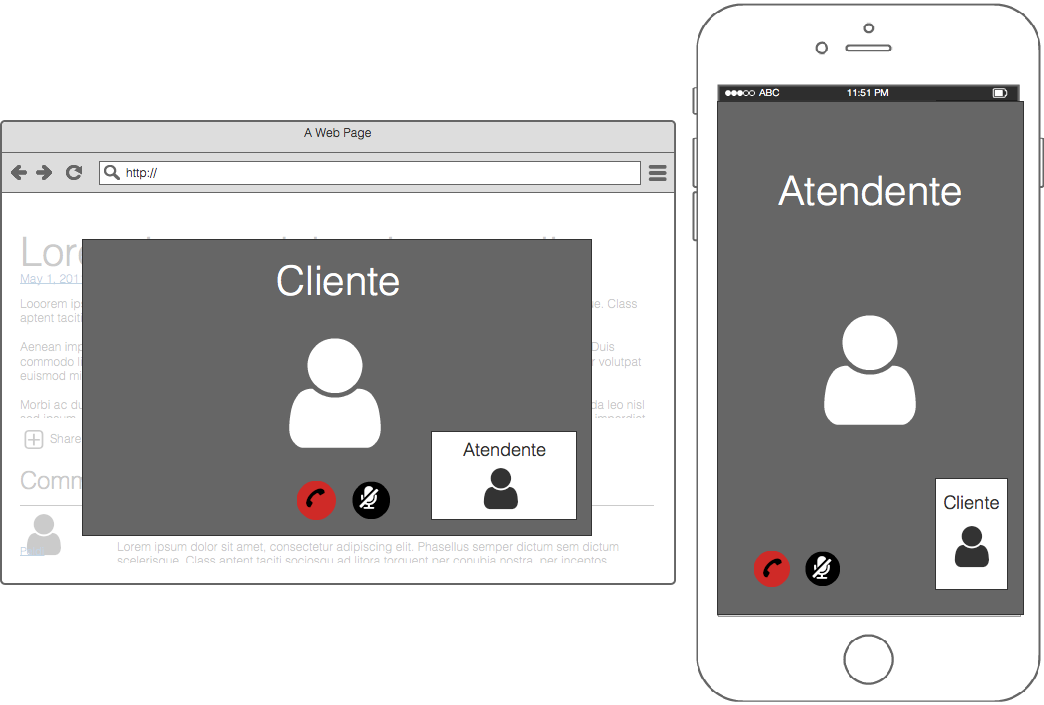
\includegraphics[scale=0.2]{figures/prototypes/videoconference.png} 
	\caption{Videoconferência entre atendente e cliente}
	\label{fig:videoconference}
\end{figure}

\section{Arquitetura}

Observamos na \autoref{fig:overview_architecture} uma visão geral da arquitetura do sistema. Notamos que o modelo utilizado é o clássico cliente-servidor.

\begin{figure}[ht!]
	\centering
		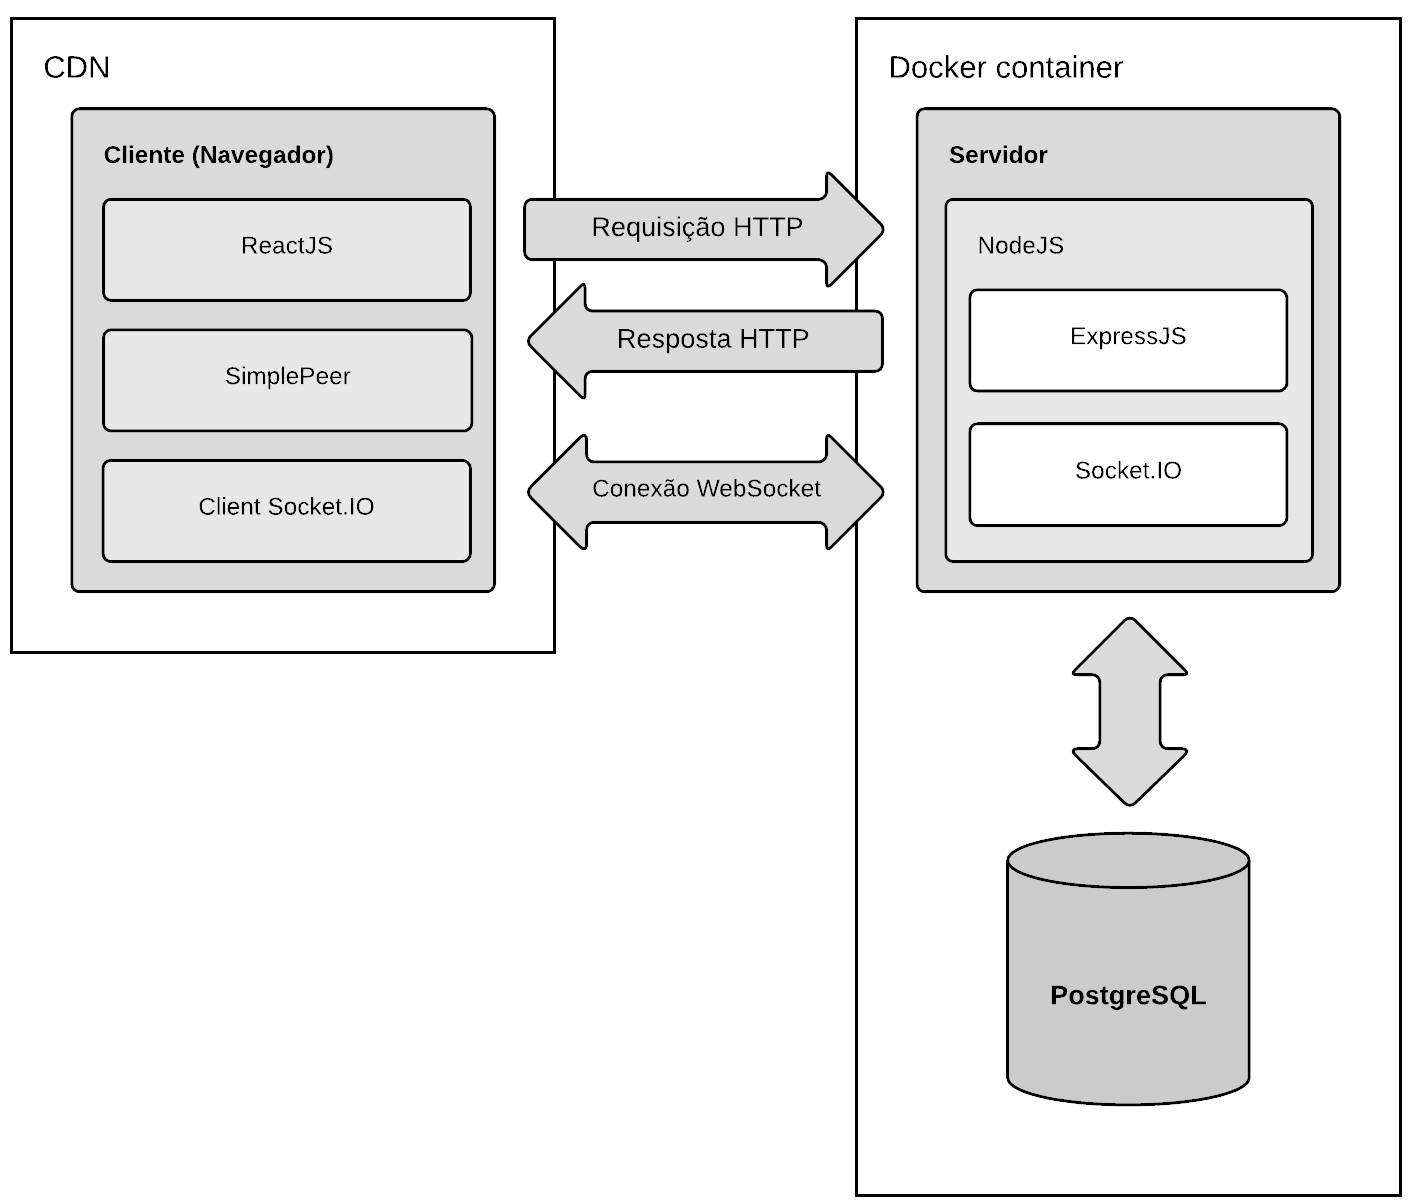
\includegraphics[scale=0.2]{figures/overview-architecture.png} 
	\caption{Arquitetura do sistema}
	\label{fig:overview_architecture}
\end{figure}

\subsection{Servidor}

Todo o \textit{back-end} foi implementado sobre a plataforma NodeJS. Essa tornou-se popular dentre os desenvolvedores nos últimos tempos devido à capacidade de executar código JavaScript fora do navegador. 

Podemos elencar três componentes mais importantes no lado do servidor. O primeiro deles é a base, uma interface de programação de aplicação (API) nos modelos da arquitetura REST, implementada com o \textit{framework} ExpressJS, utilizado para facilitar a construção de aplicações Web. O servidor da API, além de ser utilizado para salvar informações no banco de dados, também é responsável por iniciar a conexão através de \textit{sockets}.

O segundo componente é outro \textit{framework}, SocketIO, desenvolvido com o o objetivo de facilitar o \textit{upgrade} de requisições HTTP e estabelecer a comunicação através de WebSockets. Esse \textit{framework} abstrai as APIs complexas do navegador em padrões já conhecidos, fornecendo ao desenvolvedor uma outra arquitetura mais simples de usar.

Por último, temos o gerenciador de banco de dados PostgreSQL, que armazena os dados das chamadas, atendentes, administradores e clientes do sistema.

\subsection{Cliente}

O lado do cliente será sempre executado em um navegador, ou seja, foi inteiramente implementado com HTML e JavaScript. 

Utiliza o \textit{framework} React para renderizar interfaces. É baseado em composição de componentes, sendo cada um deles uma peça da interface. Esses componentes têm acesso às APIs nativas do navegador, podendo assim realizar requisições HTTP através de interfaces como AJAX.

É responsabilidade do cliente solicitar uma conexão \text{peer-to-peer} com um navegador remoto, conforme ilustrado na figura \ref{fig:peer_connection}, que remete a assuntos abordados no capítulo \ref{chap:fundamentacao}.

\begin{figure}[ht!]
	\centering
		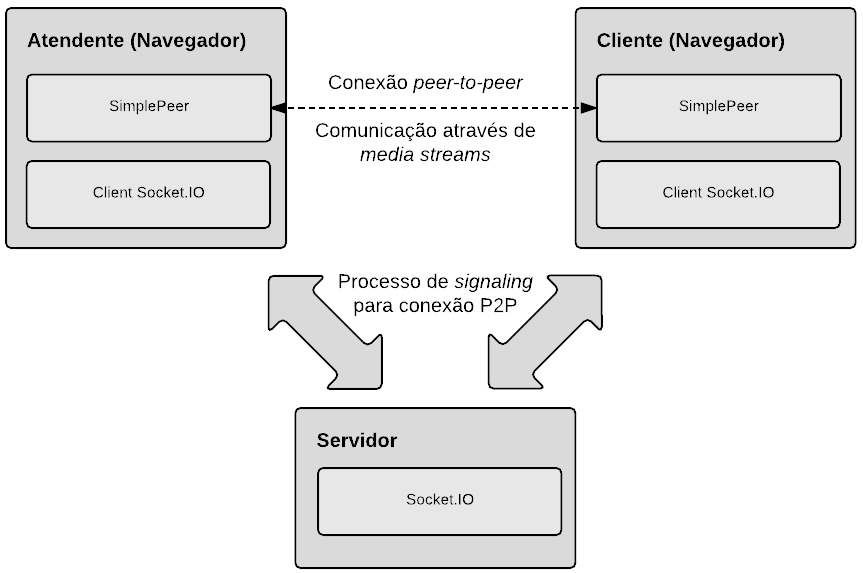
\includegraphics[scale=0.35]{figures/overview-client.png} 
	\caption{Conexão peer-to-peer através de WebSockets}
	\label{fig:peer_connection}
\end{figure}

Com a conexão estabelecida entre os dois pontos, a aplicação renderiza automaticamente uma nova tela, na qual o cliente consegue enxergar o atendente e vice-versa.

\section{Modelagem do banco de dados}

O diagrama de entidades, representado na figura \ref{fig:database_model}, contém a modelagem do banco de dados da aplicação. 

\begin{figure}[ht!]
	\centering
		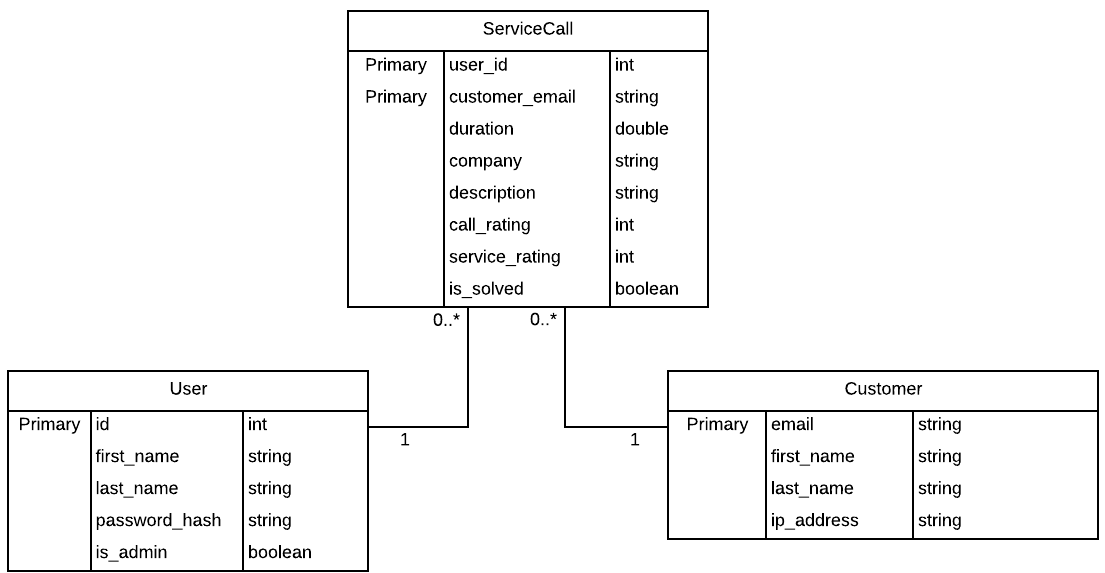
\includegraphics[scale=0.8]{figures/database-model.png} 
	\caption{Entidades do banco de dados}
	\label{fig:database_model}
\end{figure}

A entidade \textit{User} representa os atendentes do serviço de atendimento ao consumidor. Todo atendente necessita fazer login no sistema para poder criar salas e atender clientes. Esse mesmo usuário tem permissão para visualizar dados e estatísticas de chamadas.

Para representar os clientes que realizam chamadas de suporte criamos a entidade \textit{Customer}. Essa entidade não necessita de login para solicitar um atendente, visto que o objetivo do sistema é prover uma maneira fácil para pessoas obterem resolução de problemas.

Por fim, as chamadas de suporte são representadas pela entidade \textit{ServiceCall}. Essa entidade possuí o tempo de duração de atendimento e faz a relação entre atendente e consumidor. Foram adicionados também dados da chamada, como avaliação e se o problema foi resolvido ou não, para que seja possível registrar estatísticas e criar uma página com informações para os atendentes.

